\documentclass{report}
% \documentclass[12pt, a4paper]{ctexart}
\usepackage{amsmath, amsthm, amssymb, graphicx}
\usepackage{bm}
\newtheorem{definition}{Definition}[section]
\newtheorem{proposition}{Proposition}[section]
\newtheorem{lemma}{Lemma}[section]
\newtheorem{theorem}{Theorem}[section]
\newtheorem{corollary}[theorem]{Corollary}
\newtheorem{example}{Example}[section]
\newtheorem{remark}{Remark}[section]
\newenvironment{solution}{\begin{proof}[\textbf{Solution}]}{\end{proof}}
% \newtheorem{proof}{Proof}[section]
\usepackage[bookmarks=true, colorlinks, citecolor=blue, linkcolor=black]{hyperref}
\usepackage{geometry}
\usepackage{graphicx}
\counterwithin{figure}{section}
% \usepackage{graphicx, xcolor, transparent}
\usepackage{quiver, tikz-cd}
\usepackage{cite, tcolorbox}
% \usepackage{lipsum}
\geometry{left=2.54cm, right=2.54cm, top=3.18cm, bottom=3.18cm}

\title{A Note on Differential Geometry}
\author{Hifive Zheng}
\date{\today}


\begin{document}
    \maketitle


    \chapter{Geometry in Euclidean Space}

In this section, we are going to derive what a tangent vector or a cotangent vector is,
give them a good definition and have a new view on differential and derivative. \textit{(We will
ignore many detials in order to grasp the very idea instead of being lost in tedious derivation.)}

\section{Explicit Function and Implicit Equation}

It's time to clarify the difference between implicit function and explicit function!
Consider a explicit function $F: \mathbb{R}^2\to\mathbb{R}, (x,y)\mapsto z=F(x,y)$ which can be thought of a scalar field over $\mathbb{R}^2$
Esay, right? What about taking the value of $z$ as $0$? Is it a constant scalar field valued $0$? Never! There is a huge diference between $F(x,y)=0$ and $F(x,y)\equiv 0$.
The first one is a function that tells you $z\equiv 0$ whatever values $x$ and $y$ take; and the second one tells that for the specific function $z=F(x,y)$
, $F(x,y)=0$ determines a set of $(x,y)$ satisfying the equation $F(x,y)=0$.

Actually, due to our laziness and ambiguity, when we say a function $y=f(x)$ or $f(x)$, we are not really say that $y=f(x)$ or $f(x)$ is a function -
because $y=f(x)$ is a formula and $f(x)$ is a value! However, $y=f(x)$ is the definition formula of the funciton $f:x\mapsto y=f(x)$,
implying a binary relation that for a given $x$ in the defined domain, there is a unique $y$ corresponding to it (or determined).
Because a formula $y=f(x)$ defines a funciton $f$, no wonder we mixed them up! Same, $y$ is the image of $f$, which is the same as $f(x)$,
so it is always omitted.

Going back to the example we started with. \textbf{Given a formula that contains a function, if the function has been defined, then the formula is a equation;
if the function has not been defined, then we can consider the formula as the definition formula of the function.}
So, for a function $F: \mathbb{R}^2\to\mathbb{R}, (x,y)\mapsto z=F(x,y)$, what's the formula $F(x,y)=0$ means?
It means the intersection curve between the x-y coordinate plane and the scalar filed surface in the $\mathbb{R}^2\times\mathbb{R}=\mathbb{R}^3$ space.

\begin{figure}[!ht]
	\centering
	

\tikzset{every picture/.style={line width=0.75pt}} %set default line width to 0.75pt        

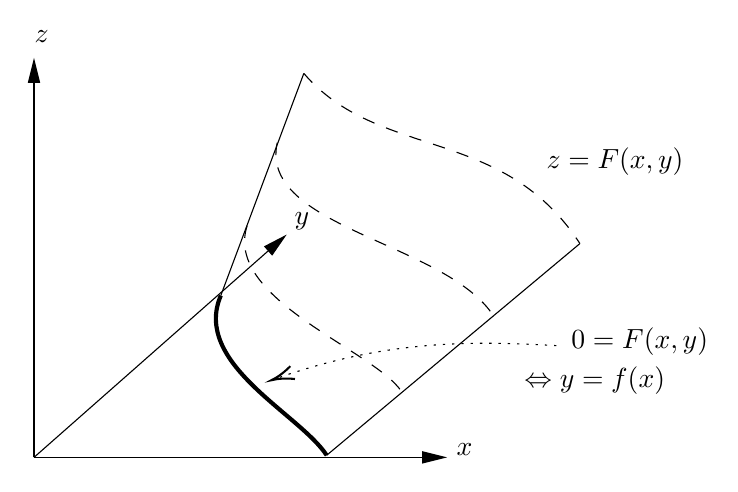
\begin{tikzpicture}[x=0.75pt,y=0.75pt,yscale=-1,xscale=1]
%uncomment if require: \path (0,300); %set diagram left start at 0, and has height of 300

%Straight Lines [id:da41514678307811437] 
\draw    (199,239.83) -- (396,239.83) ;
\draw [shift={(398,239.83)}, rotate = 180] [fill={rgb, 255:red, 0; green, 0; blue, 0 }  ][line width=0.08]  [draw opacity=0] (12,-3) -- (0,0) -- (12,3) -- cycle    ;
%Straight Lines [id:da025890045307131793] 
\draw    (199,239.83) -- (199,49.38) ;
\draw [shift={(199,47.38)}, rotate = 90] [fill={rgb, 255:red, 0; green, 0; blue, 0 }  ][line width=0.08]  [draw opacity=0] (12,-3) -- (0,0) -- (12,3) -- cycle    ;
%Straight Lines [id:da15495244964933041] 
\draw    (199,239.83) -- (319.26,133.8) ;
\draw [shift={(320.76,132.48)}, rotate = 138.6] [fill={rgb, 255:red, 0; green, 0; blue, 0 }  ][line width=0.08]  [draw opacity=0] (12,-3) -- (0,0) -- (12,3) -- cycle    ;
%Curve Lines [id:da849941590925275] 
\draw [fill={rgb, 255:red, 0; green, 0; blue, 0 }  ,fill opacity=0 ][line width=1.5]    (289,161.83) .. controls (275,194.67) and (327,218.83) .. (340,238.83) ;
%Straight Lines [id:da24207362528961096] 
\draw [fill={rgb, 255:red, 0; green, 0; blue, 0 }  ,fill opacity=0 ]   (329,54.83) -- (289,161.83) ;
%Straight Lines [id:da9090288937352464] 
\draw [fill={rgb, 255:red, 0; green, 0; blue, 0 }  ,fill opacity=0 ]   (462,136.83) -- (340,238.83) ;
%Curve Lines [id:da5116887500934504] 
\draw [fill={rgb, 255:red, 0; green, 0; blue, 0 }  ,fill opacity=0 ] [dash pattern={on 4.5pt off 4.5pt}]  (329,54.83) .. controls (365,96.83) and (425,79.83) .. (462,136.83) ;
%Curve Lines [id:da1189532235710109] 
\draw [fill={rgb, 255:red, 0; green, 0; blue, 0 }  ,fill opacity=0 ] [dash pattern={on 4.5pt off 4.5pt}]  (301.67,128.25) .. controls (290.17,163.75) and (363.17,188.25) .. (376.17,208.25) ;
%Curve Lines [id:da8449945051906733] 
\draw [fill={rgb, 255:red, 0; green, 0; blue, 0 }  ,fill opacity=0 ] [dash pattern={on 4.5pt off 4.5pt}]  (316.17,88.25) .. controls (307.17,129.25) and (397.67,136.25) .. (420.5,171.83) ;
%Curve Lines [id:da7155593188111713] 
\draw  [dash pattern={on 0.84pt off 2.51pt}]  (450.67,186) .. controls (405.79,183.36) and (366.13,183.99) .. (314.89,202.11) ;
\draw [shift={(313.33,202.67)}, rotate = 340.25] [color={rgb, 255:red, 0; green, 0; blue, 0 }  ][line width=0.75]    (10.93,-3.29) .. controls (6.95,-1.4) and (3.31,-0.3) .. (0,0) .. controls (3.31,0.3) and (6.95,1.4) .. (10.93,3.29)   ;

% Text Node
\draw (401.33,231.73) node [anchor=north west][inner sep=0.75pt]    {$x$};
% Text Node
\draw (198,33.07) node [anchor=north west][inner sep=0.75pt]    {$z$};
% Text Node
\draw (323.33,120.4) node [anchor=north west][inner sep=0.75pt]    {$y$};
% Text Node
\draw (444.67,89.4) node [anchor=north west][inner sep=0.75pt]    {$z=F( x,y)$};
% Text Node
\draw (456.67,176.07) node [anchor=north west][inner sep=0.75pt]    {$0=F( x,y)$};
% Text Node
\draw (434,194.73) node [anchor=north west][inner sep=0.75pt]    {$\Leftrightarrow y=f( x)$};


\end{tikzpicture}

	\caption{The intersection curve between the x-y coordinate plane and the scalar filed surface.}
	\label{intersection}
\end{figure}

As figure \ref{intersection} shows above, $F(x,y)=0$ determines a function $f: \mathbb{R}\to\mathbb{R}, x\mapsto y=f(x)$ if we transform the formula to the form of $y=f(x)$.


\section{Derivative and Tangent Vector}

A function $f: \mathbb{R}^2\to\mathbb{R}, (x,y)\mapsto z=f(x,y)$ is a explicit function and scalar filed over $\mathbb{R}^2$.
$f$ has good properties that we can define a derivative over it:

\begin{definition}
	For a real-valued function $f\in C^{k}: \mathbb{R}\to\mathbb{R}$, the \textbf{derivative} on $x_0\in D(f)$ is defined by:
	\[
		\left.\frac{\mathrm{d}}{\mathrm{d}x}\right|_{x_0} f :=
		\lim_{\Delta x\to 0}\frac{f(x_0+\Delta x)-f(x_0)}{t},
	\]
	for $\Delta x\in\mathbb{R}$.
\end{definition}

\begin{definition}
	Construct a function $\frac{\mathrm{d}}{\mathrm{d}x}f: C^{k}\to\mathbb{R}$ satisfying:
	\[
		\left(\frac{\mathrm{d}}{\mathrm{d}x}f\right)(x_0) :=
		\left.\frac{\mathrm{d}}{\mathrm{d}x}\right|_{x_0} f.
	\]
	$\frac{\mathrm{d}}{\mathrm{d}x}f$ is called the \textbf{derivative function}.
	It is denoted as $\frac{\mathrm{d}}{\mathrm{d}x}f\equiv f'$ simultaneously when it is clear whom to take the derivative from (always $x$).
	It is also write as $\dot{f}$ when taking the derivative from $t$.
\end{definition}

There are abundant corollaries on the field of derivative and are needless to say more. Let's turn our attention to
scalar field over $\mathbb{R}^n$, and we'll define the \textbf{derivative operator} and \textbf{directional derivative}
as well as the \textbf{gradient}. And we'll further study their geometric significance in the next section.

\begin{definition} [Parital Derivative]
	Given a function $f: \mathbb{R}^n\to\mathbb{R}, \bm{x}=(x^1,\dots,x^n)\mapsto y=f(\bm{x})$. The limitation is defined as the \textbf{partial derivative} at $\bm{x_0}$:
	\[
		\left.\frac{\partial}{\partial x^i}\right|_{\mathrm{x_0}} f:=
		\lim_{\Delta x^i\to 0}\frac{f(\dots,x_0^i+\Delta x^i,\dots)-f(\bm{x_0})}{\Delta x^i}=
		\left.\frac{\mathrm{d}}{\mathrm{d}x^i}\right|_{x^i=x_0^i} f(x_0^1,\dots,x^i,\dots,x_0^n).
	\]
\end{definition}

\begin{definition}
	\[
		\left(\frac{\partial}{\partial x^i}f\right)(\bm{x_0}):=
		\left.\frac{\partial}{\partial x^i}\right|_{\mathrm{x_0}} f
	\]
\end{definition}

\begin{theorem}[Chain Rule]
	Given a function $f: \mathbb{R}^n\to\mathbb{R}^m, \bm{x}\mapsto\mathbf{y}=f(\bm{x})$ that eats n variables and spit out m variables where $\bm{x}=(x^1,\dots,x^n), \mathbf{y}=(y^1,\dots,y^m)$.
	It can be thought of a vector $\langle f_1,\dots,f_n\rangle$ in which $f_i: \mathbb{R}\to\mathbb{R}^m, \bm{x}\mapsto y^i=f(\bm{x})$.
	All partial derivatives can be written in a maritx, which we called a \textbf{partial derivative tensor}:
	\[
		\frac{\partial f_j}{\partial x^i} = 
		\begin{bmatrix}
			\frac{\partial f_1}{\partial x^1} & \cdots & \frac{\partial f_1}{\partial x^n} \\
			\vdots & \ddots & \vdots \\
			\frac{\partial f_m}{\partial x^1} & \cdots & \frac{\partial f_m}{\partial x^n}
		\end{bmatrix}.
	\]
	Now we use vectors to represent a function chain: $\mathbf{z}=g(\mathbf{y}), \mathbf{y}=f(\bm{x})$. Then $\mathbf{z}=g(f(\bm{x}))=(g\circ f)(\bm{x})$. As can vertify,
	The partial derivative tensor of $z$ over $x$ is (here $z=g\circ f$ also):
	\begin{equation}
		\label{chain_rule}
		\frac{\partial z^k}{\partial x^i} = \frac{\partial g_k}{\partial y^j}\frac{\partial f_j}{\partial x^i},
	\end{equation}
	which is called the \textbf{Chain Rule}.
\end{theorem}

The partial derivative tensor written above is also a \textbf{Jacobian Matrix} of a vector-valued function. But isn't it better to take tensor notation?
When so, the gradient of each components can be represent more concise and intuitive!
\begin{equation}
	\label{jacobi_gradient}
	D\vec{f} = \nabla f_j = \frac{\partial f_j}{\partial x^i}.
\end{equation}

\begin{example}
	\begin{itemize}
		\item[(1)] Calculate the gradient of $f(x,y)=\sin(xy)+\frac{x^2}{1+\ln y}$ at $(\pi,1)$.
		\begin{solution}
			$\frac{\partial f}{\partial x} = y\cos(xy)+\frac{2x}{1+\ln y},
			\quad \frac{\partial f}{\partial y} = x\cos(xy)-\frac{x^2}{y(1+\ln y)^2}$.

			Then $\nabla f|_{(\pi,1)}=(\left.\frac{\partial f}{\partial x}\right|_{(\pi,1)}, \left.\frac{\partial f}{\partial y}\right|_{(\pi,1)})=
			(-1+2\pi, -\pi-\pi^2)$.
		\end{solution}
		\item[(2)] Given a composite function $z=f(x+y^2, ye^x)$, calculate $\frac{\partial z}{\partial x}$.
		\begin{solution}
			Denote that $z=f(u,v)=f(u^1(x,y),u^2(x,y))$. According to the Chain Rule:
		
			$\frac{\partial z}{\partial x}=\frac{\partial f}{\partial u^i}\frac{\partial u^i}{\partial x}=\frac{\partial f}{\partial u^1}+\frac{\partial f}{\partial u^2}ye^x$.
		\end{solution}
	\end{itemize}
\end{example}

\begin{definition}[Derivative Operator]
	For a scalar field $f: \mathbb{R}^n\to\mathbb{R}$, consider a column vector: $\bm{v}=\langle v^1,\dots,v^n\rangle$.
	Define a coordinate function $x: p\mapsto \bm{x}=x(p)\in\mathbb{R}^n$, which can be determined by $x^i: p\mapsto x^i=x^i(p)\in\mathbb{R}$, $\bm{x}=(x^1,\dots,x^n)$.
	Then the coordinate of a neighbor in $\bm{v}$ direction can be determined by a function $c(t)=\bm{x}+t\bm{v}=(x^1+tv^1,\dots,x^n+tv^n)$.

	The \textbf{derivative operator} $D_{v,p}: C^{k}\to\mathbb{R}$ over $p$ is a map satisfying:
	\[
		D_{v,p}f := \lim_{t\to 0}\frac{f(c(t))-f(\bm{x})}{t} =
		\left.\frac{\mathrm{d}}{\mathrm{d} t}\right|_{t=0} (f\circ c)
	\]
\end{definition}

By using the Chain Rule, we get $\left.\frac{\mathrm{d}}{\mathrm{d} t}\right|_{t=0} (f\circ c) = v^i \left.\frac{\partial}{\partial x^i}\right|_{p} f$.
Since this is established for $\forall x_0 \in D(f)$, we obtain:
$D_{v}f = v^i \cdot \left(\frac{\partial}{\partial x^i}f\right)$.
All the derivative operators at point $p$ constitude a set denoted by $\mathcal{D}_p(\mathbb{R}^n)$. As can be proven, $\mathcal{D}_p(\mathbb{R}^n)$ is a vector space.
All the vectors at point $p$ constitude a set denoted by $T_p(\mathbb{R}^n)$. As can be proven, $T_p(\mathbb{R}^n)$ is a vector space as well.

% we may define vector field first!

\begin{definition}[Directional Derivative]
	Construct a function $D_vf: D(f)\to\mathbb{R}$ that satisfies:
	\[
		D_{v}f := v^i\cdot \left(\frac{\partial}{\partial x^i}f\right), \quad
		\left.D_vf\right|_p := v^i\cdot \left.\frac{\partial}{\partial x^i}\right|_p f.
	\]
	This means the \textbf{directional derivative} in the direction of $\bm{v}$.
\end{definition}

At Figure \ref{dirder} we can see that $\left\{\left.\frac{\partial}{\partial x^i}\right|_p\right\}$ spans a vector space as is easy to prove.
And if we construct a map $\phi: \mathcal{D}_p(\mathbb{R}^n)\to T_p(\mathbb{R}^n)$ at point $p$, we can prove that the map is an isomorphism!
That means we can consider a vector as a directional derivative, so a vector $v$ can act on a function $f$ resulting in a real number(directional derivative) $v(f)=D_{v,p}f$ at point $p$.
A directional derivative can be considered as a vector at $p$ so we can draw it on $D(f)\in\mathbb{R}^n$.

% A proof of the isomorphism...
% The following statement is pending discussion

In the sense of isomorphism of vector spaces $T_p(\mathbb{R}^n)\simeq \mathcal{D}_p(\mathbb{R}^n)$, the standard basis $\{e_i\}$ corresponds to the set of partial derivatives $\left\{ \left.\frac{\partial}{\partial x^i}\right|_p \right\}$.
From then on, we treats them as the same thing: $\bm{v}=v^i=v^ie_i=v^i\left.\frac{\partial}{\partial x^i}\right|_p$.
Interestingly, there are different interpretations of this formula. Using Einstein summation convention, $\bm{v}$ is a combination of the bases.
Using tensor notation $e_i=\left.\frac{\partial}{\partial x^i}\right|_p=\bm{1}$ then $\bm{v}=v^i=\bm{v}\cdot\bm{1}$.

If we denote $\left.\frac{\partial}{\partial x^i}\right|_p = \left( \frac{\partial}{\partial x^1}, \dots, \frac{\partial}{\partial x^n} \right)_p$ as $\nabla$, we obtain:
\begin{equation}
	\bm{v} = \bm{v}\cdot\nabla
\end{equation}

This is quit enlightening because if we know that $\left.\frac{\partial}{\partial x^1}\right|_p$ is a unit vector in $\mathcal{D}_p(\mathbb{R}^n)$,
then $\nabla = \left.\frac{\partial}{\partial x^i}\right|_p$ forms a unit matrix, e.i. $\nabla = \bm{1}$.

\begin{figure}[!ht]
	\centering
    

\tikzset{every picture/.style={line width=0.75pt}} %set default line width to 0.75pt        

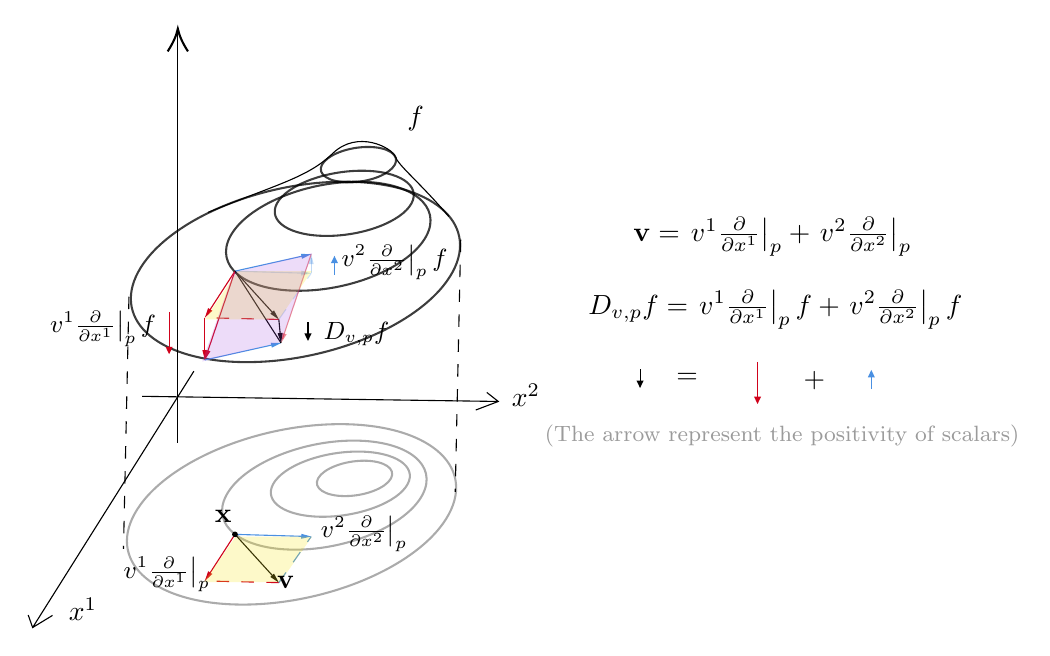
\begin{tikzpicture}[x=0.75pt,y=0.75pt,yscale=-1,xscale=1]
%uncomment if require: \path (0,324); %set diagram left start at 0, and has height of 324

%Shape: Axis 2D [id:dp392022965918875] 
\draw  (233.79,180.44) -- (156.1,303.95)(380.45,195.03) -- (208.86,192.55) (165.68,298.11) -- (156.1,303.95) -- (153.98,297.94) (374.92,190.68) -- (380.45,195.03) -- (369.6,199.15)  ;
%Straight Lines [id:da6093238245580039] 
\draw    (226.05,214.91) -- (226.05,17.44) ;
\draw [shift={(226.05,15.44)}, rotate = 90] [color={rgb, 255:red, 0; green, 0; blue, 0 }  ][line width=0.75]    (10.93,-4.9) .. controls (6.95,-2.3) and (3.31,-0.67) .. (0,0) .. controls (3.31,0.67) and (6.95,2.3) .. (10.93,4.9)   ;
%Shape: Ellipse [id:dp405330952821648] 
\draw  [color={rgb, 255:red, 0; green, 0; blue, 0 }  ,draw opacity=0.33 ][line width=0.75]  (205.09,249.42) .. controls (218.03,225.42) and (262.43,205.96) .. (304.26,205.96) .. controls (346.1,205.96) and (369.52,225.42) .. (356.59,249.42) .. controls (343.65,273.43) and (299.25,292.89) .. (257.41,292.89) .. controls (215.58,292.89) and (192.15,273.43) .. (205.09,249.42) -- cycle ;
%Shape: Ellipse [id:dp329912503849465] 
\draw  [color={rgb, 255:red, 0; green, 0; blue, 0 }  ,draw opacity=0.33 ][line width=0.75]  (249.46,240.15) .. controls (257.28,225.64) and (284.74,213.88) .. (310.81,213.88) .. controls (336.87,213.88) and (351.65,225.64) .. (343.84,240.15) .. controls (336.02,254.66) and (308.55,266.43) .. (282.49,266.43) .. controls (256.43,266.43) and (241.64,254.66) .. (249.46,240.15) -- cycle ;
%Shape: Ellipse [id:dp1514768215459963] 
\draw  [color={rgb, 255:red, 0; green, 0; blue, 0 }  ,draw opacity=0.33 ][line width=0.75]  (271.95,234.87) .. controls (276.62,226.2) and (294.92,219.17) .. (312.82,219.17) .. controls (330.72,219.17) and (341.44,226.2) .. (336.77,234.87) .. controls (332.09,243.54) and (313.79,250.58) .. (295.89,250.58) .. controls (277.99,250.58) and (267.27,243.54) .. (271.95,234.87) -- cycle ;
%Shape: Ellipse [id:dp668836996840452] 
\draw  [color={rgb, 255:red, 0; green, 0; blue, 0 }  ,draw opacity=0.33 ][line width=0.75]  (293.63,232.09) .. controls (296.17,227.38) and (306.09,223.57) .. (315.78,223.57) .. controls (325.48,223.57) and (331.28,227.38) .. (328.75,232.09) .. controls (326.21,236.8) and (316.29,240.62) .. (306.6,240.62) .. controls (296.9,240.62) and (291.1,236.8) .. (293.63,232.09) -- cycle ;
%Shape: Ellipse [id:dp5532471875103369] 
\draw  [color={rgb, 255:red, 0; green, 0; blue, 0 }  ,draw opacity=0.76 ][line width=0.75]  (206.98,132.61) .. controls (219.91,108.61) and (264.31,89.15) .. (306.15,89.15) .. controls (347.98,89.15) and (371.41,108.61) .. (358.47,132.61) .. controls (345.54,156.62) and (301.14,176.08) .. (259.3,176.08) .. controls (217.47,176.08) and (194.04,156.62) .. (206.98,132.61) -- cycle ;
%Shape: Ellipse [id:dp9452353927265793] 
\draw  [color={rgb, 255:red, 0; green, 0; blue, 0 }  ,draw opacity=0.76 ][fill={rgb, 255:red, 255; green, 255; blue, 255 }  ,fill opacity=0 ][line width=0.75]  (251.35,115.42) .. controls (259.17,100.91) and (286.63,89.15) .. (312.69,89.15) .. controls (338.75,89.15) and (353.54,100.91) .. (345.72,115.42) .. controls (337.9,129.93) and (310.44,141.69) .. (284.38,141.69) .. controls (258.32,141.69) and (243.53,129.93) .. (251.35,115.42) -- cycle ;
%Shape: Ellipse [id:dp6430572088651332] 
\draw  [color={rgb, 255:red, 0; green, 0; blue, 0 }  ,draw opacity=0.76 ][line width=0.75]  (273.83,99.57) .. controls (278.51,90.89) and (296.81,83.86) .. (314.71,83.86) .. controls (332.61,83.86) and (343.33,90.89) .. (338.65,99.57) .. controls (333.98,108.24) and (315.68,115.27) .. (297.78,115.27) .. controls (279.88,115.27) and (269.16,108.24) .. (273.83,99.57) -- cycle ;
%Shape: Ellipse [id:dp9802682025318046] 
\draw  [color={rgb, 255:red, 0; green, 0; blue, 0 }  ,draw opacity=0.76 ][line width=0.75]  (295.52,80.94) .. controls (298.06,76.23) and (307.98,72.41) .. (317.67,72.41) .. controls (327.37,72.41) and (333.17,76.23) .. (330.63,80.94) .. controls (328.1,85.64) and (318.18,89.46) .. (308.49,89.46) .. controls (298.79,89.46) and (292.99,85.64) .. (295.52,80.94) -- cycle ;
%Straight Lines [id:da11602801671001872] 
\draw  [dash pattern={on 4.5pt off 4.5pt}]  (202.51,144.58) -- (199.87,266.1) ;
%Straight Lines [id:da3663397544467202] 
\draw  [dash pattern={on 4.5pt off 4.5pt}]  (362.35,117.1) -- (359.71,238.63) ;
%Straight Lines [id:da279639923860469] 
\draw    (253.59,259.06) -- (273.38,280.83) ;
\draw [shift={(274.72,282.31)}, rotate = 227.73] [fill={rgb, 255:red, 0; green, 0; blue, 0 }  ][line width=0.08]  [draw opacity=0] (4.8,-1.2) -- (0,0) -- (4.8,1.2) -- cycle    ;
%Straight Lines [id:da8774565171359308] 
\draw [color={rgb, 255:red, 208; green, 2; blue, 27 }  ,draw opacity=1 ]   (253.59,259.06) -- (240.15,279.84) ;
\draw [shift={(239.06,281.51)}, rotate = 302.91] [fill={rgb, 255:red, 208; green, 2; blue, 27 }  ,fill opacity=1 ][line width=0.08]  [draw opacity=0] (4.8,-1.2) -- (0,0) -- (4.8,1.2) -- cycle    ;
%Straight Lines [id:da8997087652486269] 
\draw [color={rgb, 255:red, 74; green, 144; blue, 226 }  ,draw opacity=1 ]   (253.59,259.06) -- (288.31,260.06) ;
\draw [shift={(290.31,260.12)}, rotate = 181.65] [fill={rgb, 255:red, 74; green, 144; blue, 226 }  ,fill opacity=1 ][line width=0.08]  [draw opacity=0] (4.8,-1.2) -- (0,0) -- (4.8,1.2) -- cycle    ;
%Straight Lines [id:da6154119844672867] 
\draw [color={rgb, 255:red, 208; green, 2; blue, 27 }  ,draw opacity=1 ] [dash pattern={on 4.5pt off 4.5pt}]  (274.72,282.31) -- (239.06,281.51) ;
%Straight Lines [id:da2996342937898313] 
\draw [color={rgb, 255:red, 74; green, 144; blue, 226 }  ,draw opacity=1 ] [dash pattern={on 4.5pt off 4.5pt}]  (274.72,282.31) -- (290.31,260.12) ;
%Straight Lines [id:da1112796770946729] 
\draw    (253.59,132.25) -- (273.38,154.02) ;
\draw [shift={(274.72,155.5)}, rotate = 227.73] [fill={rgb, 255:red, 0; green, 0; blue, 0 }  ][line width=0.08]  [draw opacity=0] (4.8,-1.2) -- (0,0) -- (4.8,1.2) -- cycle    ;
%Straight Lines [id:da886645151103884] 
\draw [color={rgb, 255:red, 208; green, 2; blue, 27 }  ,draw opacity=1 ]   (253.59,132.25) -- (240.15,153.02) ;
\draw [shift={(239.06,154.7)}, rotate = 302.91] [fill={rgb, 255:red, 208; green, 2; blue, 27 }  ,fill opacity=1 ][line width=0.08]  [draw opacity=0] (4.8,-1.2) -- (0,0) -- (4.8,1.2) -- cycle    ;
%Straight Lines [id:da7639376209534354] 
\draw [color={rgb, 255:red, 74; green, 144; blue, 226 }  ,draw opacity=0.31 ]   (253.59,132.25) -- (288.31,133.25) ;
\draw [shift={(290.31,133.3)}, rotate = 181.65] [fill={rgb, 255:red, 74; green, 144; blue, 226 }  ,fill opacity=0.31 ][line width=0.08]  [draw opacity=0] (4.8,-1.2) -- (0,0) -- (4.8,1.2) -- cycle    ;
%Straight Lines [id:da5097974109962886] 
\draw [color={rgb, 255:red, 208; green, 2; blue, 27 }  ,draw opacity=1 ] [dash pattern={on 4.5pt off 4.5pt}]  (274.72,155.5) -- (239.06,154.7) ;
%Straight Lines [id:da5431834208380764] 
\draw [color={rgb, 255:red, 74; green, 144; blue, 226 }  ,draw opacity=0.27 ] [dash pattern={on 4.5pt off 4.5pt}]  (274.72,155.5) -- (290.31,133.3) ;
%Straight Lines [id:da7424431322975342] 
\draw [color={rgb, 255:red, 208; green, 2; blue, 27 }  ,draw opacity=1 ]   (239.06,154.7) -- (239.06,173.05) ;
\draw [shift={(239.06,175.05)}, rotate = 270] [fill={rgb, 255:red, 208; green, 2; blue, 27 }  ,fill opacity=1 ][line width=0.08]  [draw opacity=0] (4.8,-1.2) -- (0,0) -- (4.8,1.2) -- cycle    ;
%Straight Lines [id:da2537352780362212] 
\draw [color={rgb, 255:red, 74; green, 144; blue, 226 }  ,draw opacity=0.35 ]   (290.31,133.3) -- (290.31,126.06) ;
\draw [shift={(290.31,124.06)}, rotate = 90] [fill={rgb, 255:red, 74; green, 144; blue, 226 }  ,fill opacity=0.35 ][line width=0.08]  [draw opacity=0] (4.8,-1.2) -- (0,0) -- (4.8,1.2) -- cycle    ;
%Straight Lines [id:da8538391770378861] 
\draw [color={rgb, 255:red, 208; green, 2; blue, 27 }  ,draw opacity=1 ]   (253.59,132.25) -- (239.7,173.15) ;
\draw [shift={(239.06,175.05)}, rotate = 288.75] [fill={rgb, 255:red, 208; green, 2; blue, 27 }  ,fill opacity=1 ][line width=0.08]  [draw opacity=0] (4.8,-1.2) -- (0,0) -- (4.8,1.2) -- cycle    ;
%Straight Lines [id:da24860430184280746] 
\draw [color={rgb, 255:red, 74; green, 144; blue, 226 }  ,draw opacity=1 ]   (253.59,132.25) -- (288.36,124.49) ;
\draw [shift={(290.31,124.06)}, rotate = 167.43] [fill={rgb, 255:red, 74; green, 144; blue, 226 }  ,fill opacity=1 ][line width=0.08]  [draw opacity=0] (4.8,-1.2) -- (0,0) -- (4.8,1.2) -- cycle    ;
%Straight Lines [id:da25433393648592717] 
\draw [color={rgb, 255:red, 74; green, 144; blue, 226 }  ,draw opacity=1 ]   (239.06,175.05) -- (273.83,167.29) ;
\draw [shift={(275.78,166.86)}, rotate = 167.43] [fill={rgb, 255:red, 74; green, 144; blue, 226 }  ,fill opacity=1 ][line width=0.08]  [draw opacity=0] (4.8,-1.2) -- (0,0) -- (4.8,1.2) -- cycle    ;
%Straight Lines [id:da2651028764912726] 
\draw [color={rgb, 255:red, 208; green, 2; blue, 27 }  ,draw opacity=0.45 ]   (290.31,124.06) -- (276.42,164.96) ;
\draw [shift={(275.78,166.86)}, rotate = 288.75] [fill={rgb, 255:red, 208; green, 2; blue, 27 }  ,fill opacity=0.45 ][line width=0.08]  [draw opacity=0] (4.8,-1.2) -- (0,0) -- (4.8,1.2) -- cycle    ;
%Straight Lines [id:da887357681214503] 
\draw    (274.72,155.5) -- (275.6,164.86) ;
\draw [shift={(275.78,166.86)}, rotate = 264.69] [fill={rgb, 255:red, 0; green, 0; blue, 0 }  ][line width=0.08]  [draw opacity=0] (4.8,-1.2) -- (0,0) -- (4.8,1.2) -- cycle    ;
%Straight Lines [id:da9879518755298273] 
\draw    (253.59,132.25) -- (275.78,166.86) ;
%Shape: Rectangle [id:dp48139861566876485] 
\draw  [color={rgb, 255:red, 0; green, 0; blue, 0 }  ,draw opacity=0 ][fill={rgb, 255:red, 248; green, 231; blue, 28 }  ,fill opacity=0.24 ] (254.91,132.25) -- (290.58,132.25) -- (274.72,155.5) -- (239.06,155.5) -- cycle ;
%Shape: Rectangle [id:dp228264440355205] 
\draw  [color={rgb, 255:red, 0; green, 0; blue, 0 }  ,draw opacity=0 ][fill={rgb, 255:red, 165; green, 80; blue, 227 }  ,fill opacity=0.2 ] (252.85,132.87) -- (290.74,123.52) -- (275.71,166.44) -- (237.82,175.79) -- cycle ;
%Shape: Rectangle [id:dp7530585387976709] 
\draw  [color={rgb, 255:red, 0; green, 0; blue, 0 }  ,draw opacity=0 ][fill={rgb, 255:red, 248; green, 231; blue, 28 }  ,fill opacity=0.24 ] (253.96,260.12) -- (290.75,260.12) -- (275.39,282.04) -- (238.6,282.04) -- cycle ;
%Shape: Ellipse [id:dp5682659762825244] 
\draw  [color={rgb, 255:red, 0; green, 0; blue, 0 }  ,draw opacity=0 ][fill={rgb, 255:red, 0; green, 0; blue, 0 }  ,fill opacity=1 ] (252.18,259.06) .. controls (252.18,258.31) and (252.81,257.7) .. (253.59,257.7) .. controls (254.37,257.7) and (254.99,258.31) .. (254.99,259.06) .. controls (254.99,259.81) and (254.37,260.42) .. (253.59,260.42) .. controls (252.81,260.42) and (252.18,259.81) .. (252.18,259.06) -- cycle ;
%Curve Lines [id:da2976014961647424] 
\draw    (240.67,103.93) .. controls (273.87,90.33) and (288.67,87.13) .. (300.67,75.53) .. controls (312.67,63.93) and (329.27,72.73) .. (330.87,77.13) .. controls (332.47,81.53) and (341.87,88.73) .. (356.67,105.93) ;
%Straight Lines [id:da10174581755467726] 
\draw [color={rgb, 255:red, 208; green, 2; blue, 27 }  ,draw opacity=1 ]   (221.86,151.9) -- (221.86,169.25) ;
\draw [shift={(221.86,172.25)}, rotate = 270] [fill={rgb, 255:red, 208; green, 2; blue, 27 }  ,fill opacity=1 ][line width=0.08]  [draw opacity=0] (3.57,-1.72) -- (0,0) -- (3.57,1.72) -- cycle    ;
%Straight Lines [id:da8263939691535676] 
\draw [color={rgb, 255:red, 74; green, 144; blue, 226 }  ,draw opacity=1 ]   (301.51,134.1) -- (301.51,127.86) ;
\draw [shift={(301.51,124.86)}, rotate = 90] [fill={rgb, 255:red, 74; green, 144; blue, 226 }  ,fill opacity=1 ][line width=0.08]  [draw opacity=0] (3.57,-1.72) -- (0,0) -- (3.57,1.72) -- cycle    ;
%Straight Lines [id:da6821225686661974] 
\draw [color={rgb, 255:red, 0; green, 0; blue, 0 }  ,draw opacity=1 ]   (288.76,162.85) -- (288.76,156.61) ;
\draw [shift={(288.76,165.85)}, rotate = 270] [fill={rgb, 255:red, 0; green, 0; blue, 0 }  ,fill opacity=1 ][line width=0.08]  [draw opacity=0] (3.57,-1.72) -- (0,0) -- (3.57,1.72) -- cycle    ;
%Straight Lines [id:da420763728946844] 
\draw [color={rgb, 255:red, 208; green, 2; blue, 27 }  ,draw opacity=1 ]   (505.36,175.9) -- (505.36,193.25) ;
\draw [shift={(505.36,196.25)}, rotate = 270] [fill={rgb, 255:red, 208; green, 2; blue, 27 }  ,fill opacity=1 ][line width=0.08]  [draw opacity=0] (3.57,-1.72) -- (0,0) -- (3.57,1.72) -- cycle    ;
%Straight Lines [id:da7927683614331424] 
\draw [color={rgb, 255:red, 74; green, 144; blue, 226 }  ,draw opacity=1 ]   (560.18,189.1) -- (560.18,182.86) ;
\draw [shift={(560.18,179.86)}, rotate = 90] [fill={rgb, 255:red, 74; green, 144; blue, 226 }  ,fill opacity=1 ][line width=0.08]  [draw opacity=0] (3.57,-1.72) -- (0,0) -- (3.57,1.72) -- cycle    ;
%Straight Lines [id:da1481174141229029] 
\draw [color={rgb, 255:red, 0; green, 0; blue, 0 }  ,draw opacity=1 ]   (448.76,185.52) -- (448.76,179.27) ;
\draw [shift={(448.76,188.52)}, rotate = 270] [fill={rgb, 255:red, 0; green, 0; blue, 0 }  ,fill opacity=1 ][line width=0.08]  [draw opacity=0] (3.57,-1.72) -- (0,0) -- (3.57,1.72) -- cycle    ;

% Text Node
\draw (172.25,288.57) node [anchor=north west][inner sep=0.75pt]    {$x^{1}$};
% Text Node
\draw (385.75,185.15) node [anchor=north west][inner sep=0.75pt]    {$x^{2}$};
% Text Node
\draw (272.67,278.15) node [anchor=north west][inner sep=0.75pt]    {$\mathbf{v}$};
% Text Node
\draw (292.17,248.95) node [anchor=north west][inner sep=0.75pt]  [font=\small]  {${\textstyle \left. v^{2}\frac{\partial }{\partial x^{2}}\right| _{p}}$};
% Text Node
\draw (197.06,268.56) node [anchor=north west][inner sep=0.75pt]  [font=\small]  {${\textstyle \left. v^{1}\frac{\partial }{\partial x^{1}}\right| _{p}}$};
% Text Node
\draw (242.65,246.19) node [anchor=north west][inner sep=0.75pt]    {${\textstyle \mathbf{x}}$};
% Text Node
\draw (161.66,150.21) node [anchor=north west][inner sep=0.75pt]  [font=\small]  {${\textstyle \left. v^{1}\frac{\partial }{\partial x^{1}}\right| _{p} f}$};
% Text Node
\draw (302.06,118.21) node [anchor=north west][inner sep=0.75pt]  [font=\small]  {${\textstyle \left. v^{2}\frac{\partial }{\partial x^{2}}\right| _{p} f}$};
% Text Node
\draw (295.08,155.71) node [anchor=north west][inner sep=0.75pt]  [font=\small]  {$D_{v,p} f$};
% Text Node
\draw (444.33,105.13) node [anchor=north west][inner sep=0.75pt]  [font=\normalsize]  {$\mathbf{v} ={\textstyle \left. v^{1}\frac{\partial }{\partial x^{1}}\right| _{p} +\left. v^{2}\frac{\partial }{\partial x^{2}}\right| _{p}}$};
% Text Node
\draw (422.62,139.91) node [anchor=north west][inner sep=0.75pt]  [font=\normalsize]  {$D_{v,p} f={\textstyle \left. v^{1}\frac{\partial }{\partial x^{1}}\right| _{p} f+\left. v^{2}\frac{\partial }{\partial x^{2}}\right| _{p} f}$};
% Text Node
\draw (335.33,51.4) node [anchor=north west][inner sep=0.75pt]    {$f$};
% Text Node
\draw (465,180.07) node [anchor=north west][inner sep=0.75pt]    {$=$};
% Text Node
\draw (526.33,179.13) node [anchor=north west][inner sep=0.75pt]    {$+$};
% Text Node
\draw (401.67,204.89) node [anchor=north west][inner sep=0.75pt]  [font=\footnotesize,color={rgb, 255:red, 155; green, 155; blue, 155 }  ,opacity=1 ] [align=left] {(The arrow represent the positivity of scalars)};


\end{tikzpicture}

    \caption{A vector and its derivatives}
    \label{dirder}
\end{figure}

\begin{definition}[Gradient]
	$\nabla$ is a \textbf{differential operator} at point $p$. $f$ is a function defined over $\mathbb{R}^n$. The gradient of $f$ at $p$ is defined by:
	\[\mathbf{grad}f:=\nabla f\]

	And $\nabla$ acting on $f$ is defined by:
	\[\nabla f:=\left.\frac{\partial}{\partial x^i}\right|_p f\]
\end{definition}

\begin{proposition}
	Direction derivative (unit) along the gradient is larger.
	\begin{proof}
		Given a unit vector $\bm{v}$ at point $p$ that $\|\bm{v}\|=1$. The directional derivative
		\[
			D_{v,p}f = \bm{v}(f) = (\bm{v}\cdot\nabla)(f) = \bm{v}\cdot(\nabla f).
		\]
		Because
		\[
			\bm{v}\cdot(\nabla f) = \|\bm{v}\|\|\nabla f\|\cos\theta\leq \|\nabla f\|=\|\mathbf{grad}f\|,
		\]
		taken the equality when and only when $\bm{v}=\lambda(\mathbf{grad}f)$, where $\lambda\in\mathbb{R}$.
	\end{proof}
\end{proposition}


There is something to note (to be change):

\begin{itemize}
	\item[(1)] There are at least two notations of denoting the derivative over $p$:
		$\left.\frac{\mathrm{d}}{\mathrm{d}x}\right|_p f$ and $\frac{\mathrm{d}}{\mathrm{d}x}f(p)$.
		We choose the first one as another one causes some ambiguity. The derivative at $p$ is a map $C^{\infty}\to \mathbb{R}$
		which eats a function and spit out a real number. And the second one seems that $f$ eats $p$ and spit out a real number first
		as if the derivative acts on $\mathbb{R}$! Right now $\left.\frac{\mathrm{d}}{\mathrm{d}x}\right|_p$ is just the very function defined
		over $p$ and its neighborhood, but if we pass through all the point in the domain we obtain a function from $\mathbb{R}$ to $\mathbb{R}$!
		
		\begin{definition}[Derivative Function $\frac{\mathrm{d}}{\mathrm{d}x}f$]
			Construct a function $\frac{\mathrm{d}}{\mathrm{d}x}f: \mathbb{R}\to\mathbb{R}$ satisfying:
			\[\left(\frac{\mathrm{d}}{\mathrm{d}x}f\right)(p) := \left.\frac{\mathrm{d}}{\mathrm{d}x}\right|_p f,\]
			which shares the same domain with $f$. $\frac{\mathrm{d}}{\mathrm{d}x}f$ is called the \textbf{derivative function}.
            \label{derf}
		\end{definition}

		\begin{example}
			Calculate the derivative of the function $f(x)=x^2$
			\begin{solution}
			Let $c(t)=(p+vt)$.
			\[
				\left.\frac{\mathrm{d}}{\mathrm{d}x}\right|_p f =
				\lim_{t\to 0}\frac{(p+vt)^2-p^2}{t} =
				\lim_{t\to 0}(2vp+v^2t) = 2vp + o(t) = 2vp.
			\]
			
			So $\frac{\mathrm{d}}{\mathrm{d}x}f$ satisfies:
			\[
				\left(\frac{\mathrm{d}}{\mathrm{d}x}f\right)(p) =
				\left.\frac{\mathrm{d}}{\mathrm{d}x}\right|_p f = 2vp,
				\quad \forall p \in D(f).
			\]		
			\end{solution}
		\end{example}

		Definition \ref{derf} seems to be redundant because we see no difference in numerical values.
		But we shall keep in mind that derivative function is a constructed function. It assigns
		a derivative value to each point but is defined by $\left.\frac{\mathrm{d}}{\mathrm{d}x}\right|_p$, that is,
		a map from the origin function to a derivative value over a certain point $p$.

		So how shall we view derivatives? A value, a map, or a real-valued function? The difference between the first two point
		is the same that $y$ between $y(x)$ in the function $y=y(x)$. So let's clarify it:
		\begin{itemize}
			\item[(i)] $\left.\frac{\mathrm{d}}{\mathrm{d}x}\right|_p$ is a map $C^{\infty}\to\mathbb{R}$ called a \textbf{derivative operator}.
			\item[(ii)] $\left.\frac{\mathrm{d}}{\mathrm{d}x}\right|_p f$ is the image of the derivative operator, which called a \textbf{derivative}.
			\item[(iii)] $\left(\frac{\mathrm{d}}{\mathrm{d}x}f\right)$ is a real-valued function called a \textbf{derivative function}.
			\item[(iv)] $\left(\frac{\mathrm{d}}{\mathrm{d}x}f\right)(p)$ is the image of the derivative function, which is the same as (ii) on the same point.
		\end{itemize}

	\item[(2)] Notice that I use $c(t)=x_0+vt$ instead of $x_0+\Delta x$, because I want to introduce the parameter $t$ into consideration.
		The reason is, if we talk about the process of taking the derivative, the picture in mind is that a point is approaching $p$ gradually.
		Simply use $x \in D(f) \subseteq \mathbb{R}$ is a little vague because we think of $x$ the axis function of point $p$ ($x_0=x(p)$), and
		we will see later that it fails to work when it comes to implicit function or multivariate function. So, we need another purer quantity to
		measure and represent the limit process.
\end{itemize}

\[
	\left.\frac{\mathrm{d}}{\mathrm{d}x}\right|_p f =
	\left.\frac{\mathrm{d}}{\mathrm{d}x}\right|_{t=0} (f\circ c) =
	v \left.\frac{\mathrm{d}}{\mathrm{d}x}\right|_p f
\]

In $y=f(x)$

\begin{definition}[Name]
    Nothing. 
\end{definition}


% https://q.uiver.app/#q=WzAsNCxbMiwxLCJVIl0sWzQsMiwiXFxtYXRoYmJ7Un0iXSxbMCwxLCJcXG1hdGhiYntSfXxfdCJdLFs0LDAsIlxcbWF0aGJie1J9Il0sWzIsMCwiYyh0KSJdLFswLDEsImYiLDJdLFswLDMsIkRfdmZ8X3AiXSxbMiwzLCJcXGxlZnQuXFxmcmFje1xcbWF0aHJte2R9fXtcXG1hdGhybXtkfXR9XFxyaWdodHxfe3Q9MH1mKGModCkpIiwwLHsiY3VydmUiOi0zfV0sWzUsNiwiRF92IiwyLHsic2hvcnRlbiI6eyJzb3VyY2UiOjIwLCJ0YXJnZXQiOjIwfX1dXQ==
\[\begin{tikzcd}[row sep=large]
	&&&& {\mathbb{R}} \\
	{\mathbb{R}|_t} && U \\
	&&&& {\mathbb{R}}
	\arrow["{\left.\frac{\mathrm{d}}{\mathrm{d}t}\right|_{t=0}f(c(t))}", curve={height=-18pt}, from=2-1, to=1-5]
	\arrow["{c(t)}", from=2-1, to=2-3]
	\arrow[""{name=0, anchor=center, inner sep=0}, "{D_vf|_p}", from=2-3, to=1-5]
	\arrow[""{name=1, anchor=center, inner sep=0}, "f"', from=2-3, to=3-5]
	\arrow["{D_v}"', shorten <=4pt, shorten >=4pt, Rightarrow, from=1, to=0]
\end{tikzcd}\]


\section{Derivative and Tangent Vector}
\section{Differential and Cotangent Vector}
\section{Curve Theory and Surface Theory}
\section{Analytic Geometry}


    \chapter{Geometry in Oblique Coordinate System}
    \section{Covariant and Contravariant}

    \chapter{Geometry as a Manifold}


    \begin{thebibliography}{99}
        \bibitem{1}J.L. Bell, M. Machover, "A course in mathematical logic" , North-Holland (1977)
        \bibitem{2}Binary relation. Encyclopedia of Mathematics.
        \bibitem{3}Mapping. Encyclopedia of Mathematics.
    \end{thebibliography}

\end{document}